\documentclass{beamer}

\newcommand{\versionNumber}{1.1}
\newcommand{\lastEditAuthor}{Illya Starikov}

% __ Draft   __ Proposed  __ Validated  __ Approved
\newcommand{\documentStatus}{Proposed}


\EdefRot{13}\joke{maybe if we git gud, we'll use ROT26.}
\newcounter{tools}

\title{Camelot Progress Presentation}
\subtitle{Software Engineering}
\author{Ian Howell, Hunter Mathews, Illya Starikov, William Thurman, Zachary Wileman (\textit{Server Team \#1})}
\date{March 24\textsuperscript{th}, 2017}
\institute{Missouri University of Science and Technology}

\begin{document}
\maketitle


% Zachary Wileman
\begin{frame}
    \frametitle{About the Camelot Server}
    \begin{itemize}
        \item Camelot is an asynchronous \textit{Python3} server.
        \item The server is housed on a Raspberry Pi (as provided by Ian Howell) so that the client team will be able to interact and test their code on it (assuming the server is up and running) and also so that interaction with the server can be done remotely.
        \item The database is being tackled specifically by a module in Python called \textit{psycopg2} which uses \textit{PostgreSQL}.
        \item All communication between the server and client applications is done via \textit{JSON} encoded data.
    \end{itemize}
\end{frame}


% Zachary Wileman
\begin{frame}
    \frametitle{Camelot Inspiration}

    \begin{figure}
        \centering
        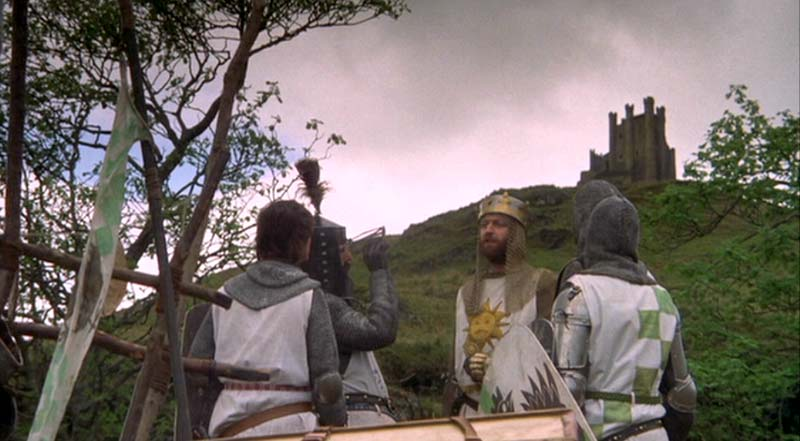
\includegraphics[width=\textwidth]{images/camelot}
        \caption{``On second thought, let's not go to Camelot. 'Tis a silly place.'' — Arthur, Monty Python}
        \label{fig:camelot}
    \end{figure}
\end{frame}


% William Thurman
\begin{frame}
    \frametitle{What Has Worked Well}
    Below are some of the things that have worked well for us up to this point.

    \begin{description}[<+->]
        \item[Teamwork] Task delegation and team work has made us able to accomplish more, in less time. Having teammates with a wide array of complementing skills and backgrounds.
        \item[Meetings] Our meetings have been productive, where topics such as documentation, implementation details, and how to change the users this time are discussed.
        \item[Changes] Sometimes when you innovate, you make mistakes (i.e. choices for users$\ldots$). It is best to admit them quickly, and get on with improving your other innovations. % — Steve Jobs
        \item[Tools] By picking some of the best tools (Github, \LaTeX{}, PostgreSQL), it has made for a much better workflow.
    \end{description}
\end{frame}


% Illya Starikov
\begin{frame}
    \frametitle{Past Changes}
    Below are past decisions that if we could change, we would. \pause

    \begin{itemize}
        \item
        \item
        \item
        \item
        \item
        \item
        \item
        \item
        \item
        \item
        \item
    \end{itemize}
\end{frame}

\begin{frame}
    \frametitle{Past Changes}
    Below are past decisions that if we could change, we would.

    % This is intentionally an MLG frog
    \centering
    \animategraphics[loop, controls, width=.75\linewidth]{12}{images/frog-}{0}{39}
\end{frame}

% Illya Starikov
\begin{frame}
    \frametitle{Tools \presentcount{tools}}
    A summary of some of the tools we're using/enjoying.

    \begin{itemize}
        \item Server code is written in Python3.
        \begin{itemize}
            \item Documentation is written in Doxygen.
        \end{itemize}

        \item All development is on Github.
        \begin{itemize}
            \item This includes meeting notes, documentation, and all production code (i.e. database and server).
            \item Github issues/milestones for task management.
            \item Contributions to make sure even workload.
        \end{itemize}

        \item All documentation/presentation is written in \LaTeX{}.
        \item Using ProgreSQL for the database.
        \item Using Discord for team/client chat -- by any memes necessary.
    \end{itemize}
\end{frame}


% Illya Starikov
\hugeslide{Documentation Demo}


% Ian Howell
\begin{frame}[fragile,c]
    \frametitle{Tools \presentcount{tools}}

    Python enables easy server setup.

    \begin{lstlisting}[style=cpython]
    def main():
        server = ThreadedTCPServer(("0.0.0.0", 9009), ThreadedTCPRequestHandler)
        ip, port = server.server_address
        server.socket.listen(10)

        server_thread = threading.Thread(target=server.serve_forever)
        server_thread.dameon = True
        server_thread.start()
        print("Server loop running in thread:", server_thread.name)

        try:
            # Loop forever
            while True:
                pass
        except KeyboardInterrupt:
            print("Cleaning up server..")
            server.shutdown()
            server.server_close()
            print("Done! Goodbye")

    \end{lstlisting}
\end{frame}


% Ian Howell
\hugeslide{Server Demo}


% Illya Starikov
\hugeslide{Github Demo}


% William Thurman
\begin{frame}
    \frametitle{Challenges}
    We have encountered three big challenges so far.

    \begin{enumerate}[<+->]
        \item Communication between the client and server teams.
        \item Direction and vision of the product.
        \item Learning curve of tools, teammates, and project.
    \end{enumerate}

    \begin{block}{Description \& Solution}
        \only<1>{Even though we have set up a system for communicating between the client and server teams (Discord), there is little to no talk between the teams. \textit{Solution: Communicate more..?}}
        \only<2>{Although there is an established, core vision (IRC clone), working out the details has proven to be difficult. \textit{Solution: Break it down to basic principles and work with teammates.}}
        \only<3>{Because we're relatively new to each other, and are unaware of each other's skill sets, assigning tasks becomes tricky. Also learning how to implement new things can be difficult. \textit{Always be sure teammates are comfortable with the tasks they're given.}}
    \end{block}
\end{frame}


% Illya Starikov
\begin{frame}
    \frametitle{Extras}

    \begin{itemize}
        \item Encryption.
        \begin{itemize}
            \item Still debating if we'll be using ROT13 (\joke) or an in-house, post-quantum cryptographic hash function using a multivariate-quadratic public-key signature system.
        \end{itemize}

        \item Open source \pause at the end of the semester.
        \item Full documentation guide courtesy of Doxygen.
    \end{itemize}
\end{frame}


% Hunter Mathews
\begin{frame}
    \frametitle{Current and Future Plans}

    \begin{enumerate}
        \item Consolidate the client and server teams to get unified protocol and systems specification document.
        \item Finish coding the actual chatroom.
        \begin{itemize}
            \item Server
            \item Database
            \item Script to automate a chatroom environment
        \end{itemize}

        \item Finish documenting the chatroom (possibly API guide).

        \pause
        \item $\cdots$
        \item Profit
    \end{enumerate}
\end{frame}


% Illya Starikov
\begin{frame}
    \frametitle{In Closing}

    Spam Illya with all questions, comments, and insults.
    \begin{description}
        \item[\faGithub]  \href{https://github.com/IllyaStarikov}{\nolinkurl{@IllyaStarikov}}
        \item[\faComment] \href{mailto:starikov@mst.edu}{\nolinkurl{starikov@mst.com}}
    \end{description}

    Special thanks to our awesome team.
    \begin{description}
        \item[\faUser] Ian Howell
        \item[\faUser] Hunter Mathews
        \item[\faUser] Illya Starikov
        \item[\faUser] William Thurman
        \item[\faUser] Zachary Wileman
    \end{description}
\end{frame}

\end{document}
